\chapter{果蝇行为识别服务网站的系统设计}

果蝇识别学是动物行为学中的重要组成部分,而自动化的分析果蝇行为对果蝇行为学的研究有重要意义。虽然不同实验室的果蝇研究环境不尽相同,但是果蝇的身体特征相对比较简单、个体之间的差异性并不明显,因而给统一的分析方法提供了可能。在解决了果蝇环境的差异对果蝇行为识别带来的困难后,可以考虑将果蝇行为识别系统推广至其他果蝇拍摄环境。为此,本文专门开发了一个基于果蝇行为识别的网站,通过在网站上提交果蝇视频,并下载识别的结果,实现自动化的果蝇行为识别。果蝇行为识别网站服务方面,主要工作包括两部分:果蝇行为识别程序和网站建设。

\section{果蝇行为识别程序}

果蝇行为识别程序的主要目标在于,通过自动化的果蝇行为分析算法,分析输入的果蝇行为视频,并将分析的结果输出。果蝇行为识别程序希望提供尽可能方便的接口,和灵活可变的配置参数,以便其他程序的调用。下面将介绍果蝇行为识别程序的模块和开发环境。

\subsection{果蝇行为识别的模块结构}

果蝇行为自动化分析主要分为几个模块:活动台的分割、果蝇身体的提取和追踪、果蝇特征的提取、果蝇行为识别。对应到程序中,果蝇行为识别程序主要划分为如图~\ref{fig:fly_detection_procedure2}所示的几个模块,各模块的功能分别如下:
\begin{description}
\item[活动台的分割] 输入包含多个果蝇活动台的视频,输出多个包含单独果蝇活动台的视频,以及对应活动台视频的相关信息,包括:果蝇活动台的中心、果蝇活动台的大小、果蝇活动台移入视频的时间、果蝇活动台移出视频的时间;其中,模块可以输出csv格式的文件,用来保存切分视频的结果;
\item[果蝇身体的提取和追踪] 输入包含单个果蝇活动台的视频,输出果蝇活动台在整个视频中的位置和大小、果蝇身体的尺寸、视频中每一帧果蝇身体和翅膀的区域、每只果蝇身体的轮廓;其中,模型将果蝇的背景模型保存成文件,以方便以后使用;
\item[果蝇特征的提取] 输入果蝇行为视频和果蝇身体提取和追踪模块的结果,输出每一帧中每只果蝇特征点的位置,以及根据果蝇特征点计算得到的果蝇姿态;此外,该模块还可以输出果蝇的速度、加速度等运动信息,并将全部的特征保存到文件;
\item[果蝇行为识别] 输入每只果蝇的位置信息、姿态信息,输出果蝇在整个时间段的行为分析结果。此外,模块还可以输出果蝇行为的特征。
\end{description}

\begin{figure}
\centering
\begin{tikzpicture}
\node [block, text width=10em] (split_chambers) {\heiti 果蝇活动台分割};
\node [block, text width=10em, below = 0.5cm of split_chambers] (extract_contour) {\heiti 果蝇身体轮廓提取};
\node [block, text width=10em, below = 0.5cm of extract_contour] (feature_extract) {\heiti 果蝇特征提取};
\node [block, text width=10em, below = 0.5cm of feature_extract] (behavior_detect) {\heiti 果蝇行为分析};

\path [arrow] (split_chambers) -- (extract_contour);
\path [arrow] (extract_contour) -- (feature_extract);
\path [arrow] (feature_extract) -- (behavior_detect);
\end{tikzpicture}
\caption{果蝇行为识别自动化分析流程}
\label{fig:fly_detection_procedure2}
\end{figure}

\subsection{果蝇行为识别程序的开发和编译环境}

果蝇行为识别程序主要部署在Linux操作系统下,其开发环境的主要依赖关系包括:
\begin{itemize}
\item OpenCV 2.4.x
\item CMake >= 3.0
\end{itemize}

OpenCV被广泛的应用在果蝇行为识别程序中\cite{itseez2015opencv,itseez2014theopencv}。OpenCV的全称Open Source Computer Vision Library,是一个免费、开源的计算机视觉方面的库,该库以BSD开源软件协议发布,提供了大量的计算机图形学中的基本操作接口,如视频、图像的IO操作、基础的图形学操作如色域转换、高级的图像特征算法如方向梯度直方图(Histogram of oriented gradient,HOG)算法\cite{dalal2005histograms}、尺度不变特征变换(Scale-invariant feature transform,SIFT)算法\cite{lowe1999object}等,以及部分计算机学习库,如SVM等。此外,OpenCV还兼容不同的平台,可以方便的部署到Windows、Linux等系统上。本文使用了稳定版本的OpenCV 2.4.x,主要利用OpenCV库提供的图形学操作进行图形的基本处理,以及机器学习库进行测试等。

对于果蝇行为识别程序而言,果蝇行为视频的处理大概能做到接近实时,即程序运行的时和果蝇视频的长度在同一个量级。和其他果蝇行为分析系统相比,该程序的运行速度并不算慢\cite{dankert2009automated},但是仍然存在较大的发展空间。对于一个摄像头,一般会同时拍摄超过20个果蝇活动台,这就给程序处理带来较大的压力。为此,在维持现有算法基本不变的情况下,可以从OpenCV库的选择入手。目前,OpenCV的最新稳定版本为 2.4.13,但是最新的开发版本已经到了 3.2.0。最新的3.2.0版本除了提供更开放的计算机图形学算法外,还为大部分的计算机图形学操作、矩阵运算等提供了GPU运算接口,对于大量的计算机图形学操作,可以大大提高程序运行的效率。

在程序的编译方面,使用CMake作为程序的make工具,并使用gcc编译器,对果蝇行为识别程序。编译完成后,得到可执行程序DetectFly,通过命令行参数指定输入的视频、果蝇行为视频的类型(打架、求偶)、输出结果的文件名等。可执行程序通过分析果蝇视频,将果蝇的行为输出到特定的文件中。外部程序可以通过调用可执行程序,得到果蝇行为视频中果蝇的所有行为。

\section{果蝇行为识别网站}

在果蝇行为自动分析程序DetectFly的基础上,本文搭建了果蝇行为自动分析的网站,对外提供果蝇行为识别服务。果蝇行为识别网站提供了用户注册、用户登录、果蝇行为识别任务的添加、果蝇行为识别任务结果下载等功能。下面简单介绍果蝇行为识别的自动化分析网站。

\subsection{网站的功能介绍}

果蝇行为识别网站的链接:\url{http://gu.ee.tsinghua.edu.cn/drosophila}。目前,网站主要包含以下功能:用户的注册、用户登录、果蝇行为视频任务的创建、果蝇行为视频上传、果蝇行为视频分析结果下载等模块。

果蝇行为识别网站存在用户管理功能。果蝇行为识别需要大量的计算资源,因而对用户的使用需要一定的条件,以便进行资格审查。首先,需要用户进行注册,只有注册用户才能使用网站提供的果蝇行为识别功能。网站的注册页面如图~\ref{fig:website_register}所示,用户需要提供包括姓名、研究机构、电子邮箱等基本信息,以便进一步联系。

\begin{figure}
\centering
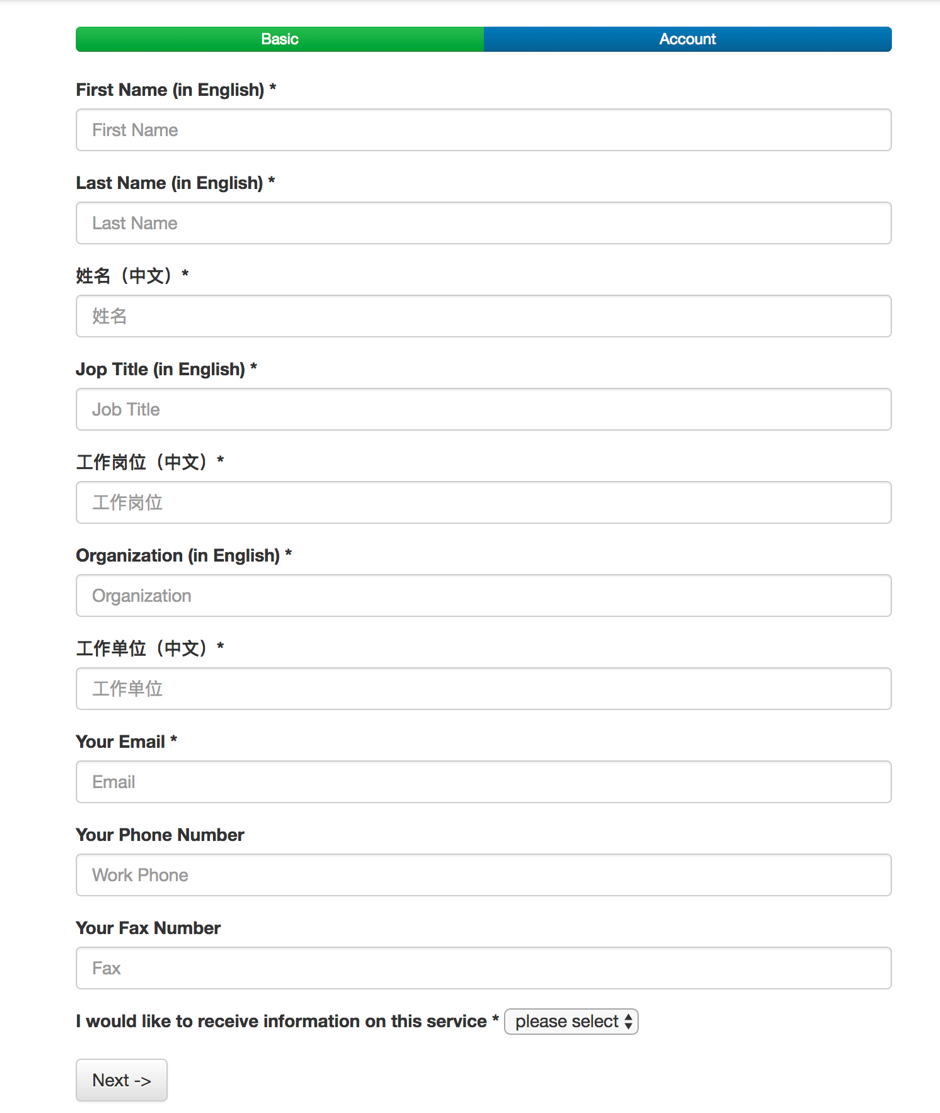
\includegraphics[width=0.8\textwidth]{website_register}
\caption{果蝇行为识别网站的注册}
\label{fig:website_register}
\end{figure}

在用户提交注册申请后,网站后台会给管理员发送邮件,等待管理员确认用户资格后,用户可以正常登陆和使用网站提供的果蝇行为识别服务。网站的登录页面如图~\ref{fig:website_login}所示。

\begin{figure}
\centering
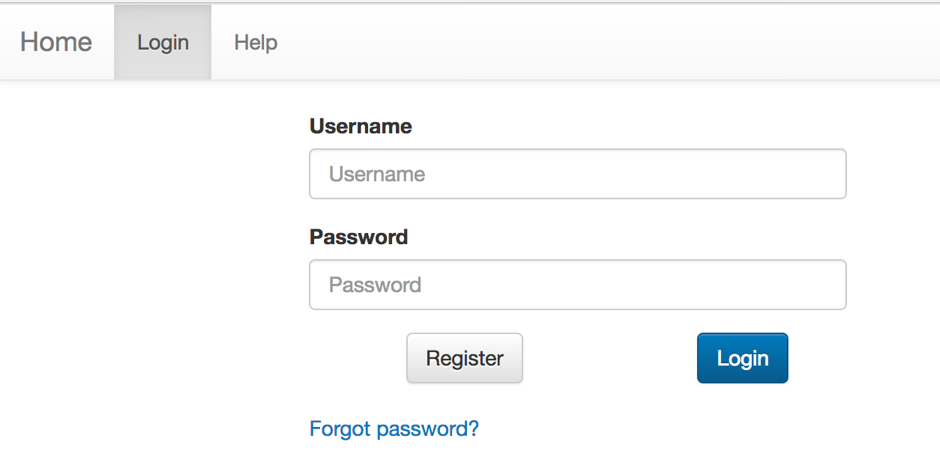
\includegraphics[width=0.8\textwidth]{website_login}
\caption{果蝇行为识别网站的登录}
\label{fig:website_login}
\end{figure}

完成登录后,可以创建果蝇行为识别任务,并上传果蝇行为视频。图~\ref{fig:website_new_mission}界面显示了创建果蝇行为识别任务的界面,目前,网站支持2种果蝇行为识别任务:打架行为和求偶行为。创建任务时,需要选定果蝇行为识别的任务类型、创建的任务名称,还支持对任务进行简单的评注,以便日后查找。对于已经完成的任务,还提供了不同的过滤列表,以便用户查询。过滤列表有以下4种:
\begin{itemize}
\item All - 全部任务列表
\item Failed - 失败的任务列表
\item Succeeded - 成功的任务列表
\item Incomplete - 未完成任务列表
\end{itemize}

\begin{figure}
\centering
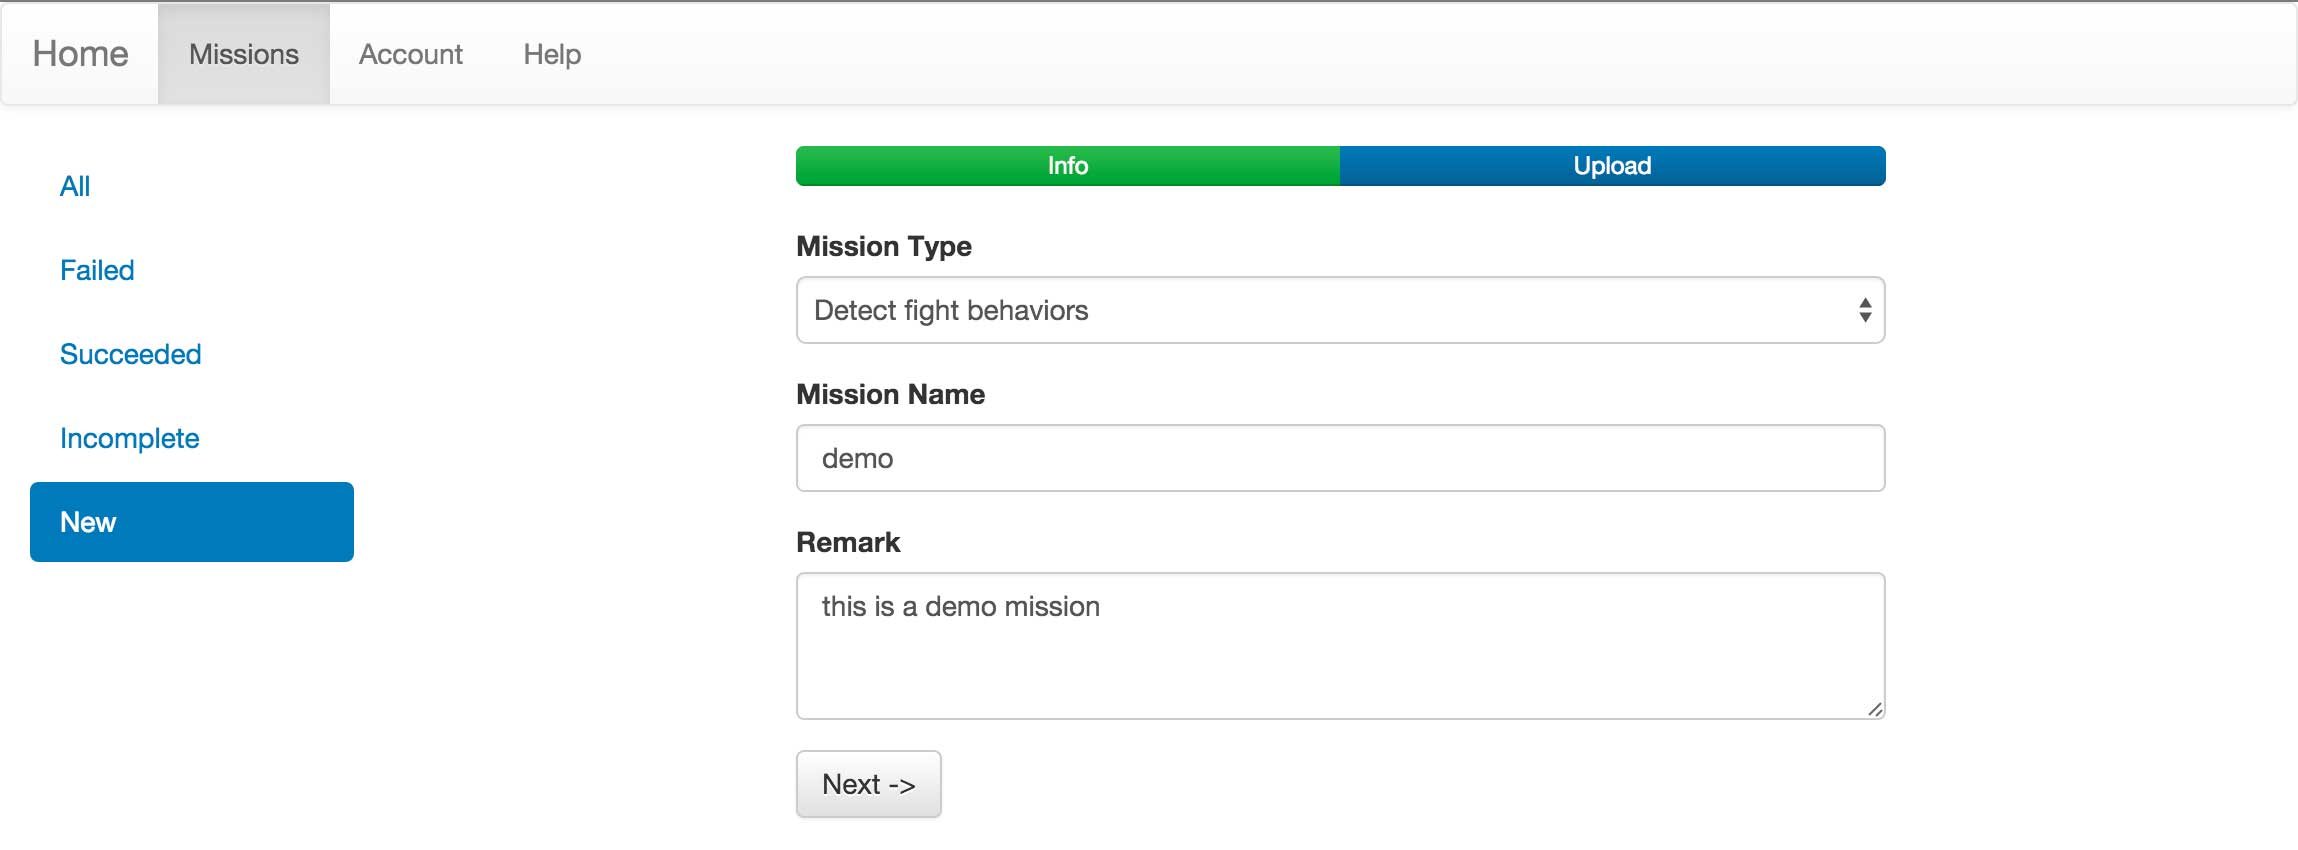
\includegraphics[width=0.8\textwidth]{website_new_mission}
\caption{创建果蝇行为识别任务}
\label{fig:website_new_mission}
\end{figure}

在完成任务创建后,需要上传果蝇行为视频。果蝇行为视频文件的大小较大,此步骤需要花费一定时间。一般来说,错误的果蝇活动台分割会给后续的果蝇行为识别任务带来难以预计的结果,这会给网站带来大量无用的计算,并消耗用户大量的时间。在综合考虑后,网站要求用户自行进行果蝇活动台的分割任务,同时要求上传的果蝇行为视频为包含一个单独的果蝇活动台的果蝇行为视频。如图~\ref{fig:website_new_mission}所示,视频文件上传完成后,点击"submit"即可提交果蝇分析任务。任务状态[Mission State]会有如下几种:
\begin{itemize}
\item Pending – 任务正在等待被处理
\item Processing – 任务正在处理中(这一步是计算过程,需要等待较长时间)
\item Succeeded – 任务处理完成
\item Failed – 任务处理失败
\end{itemize}

\begin{figure}
\centering
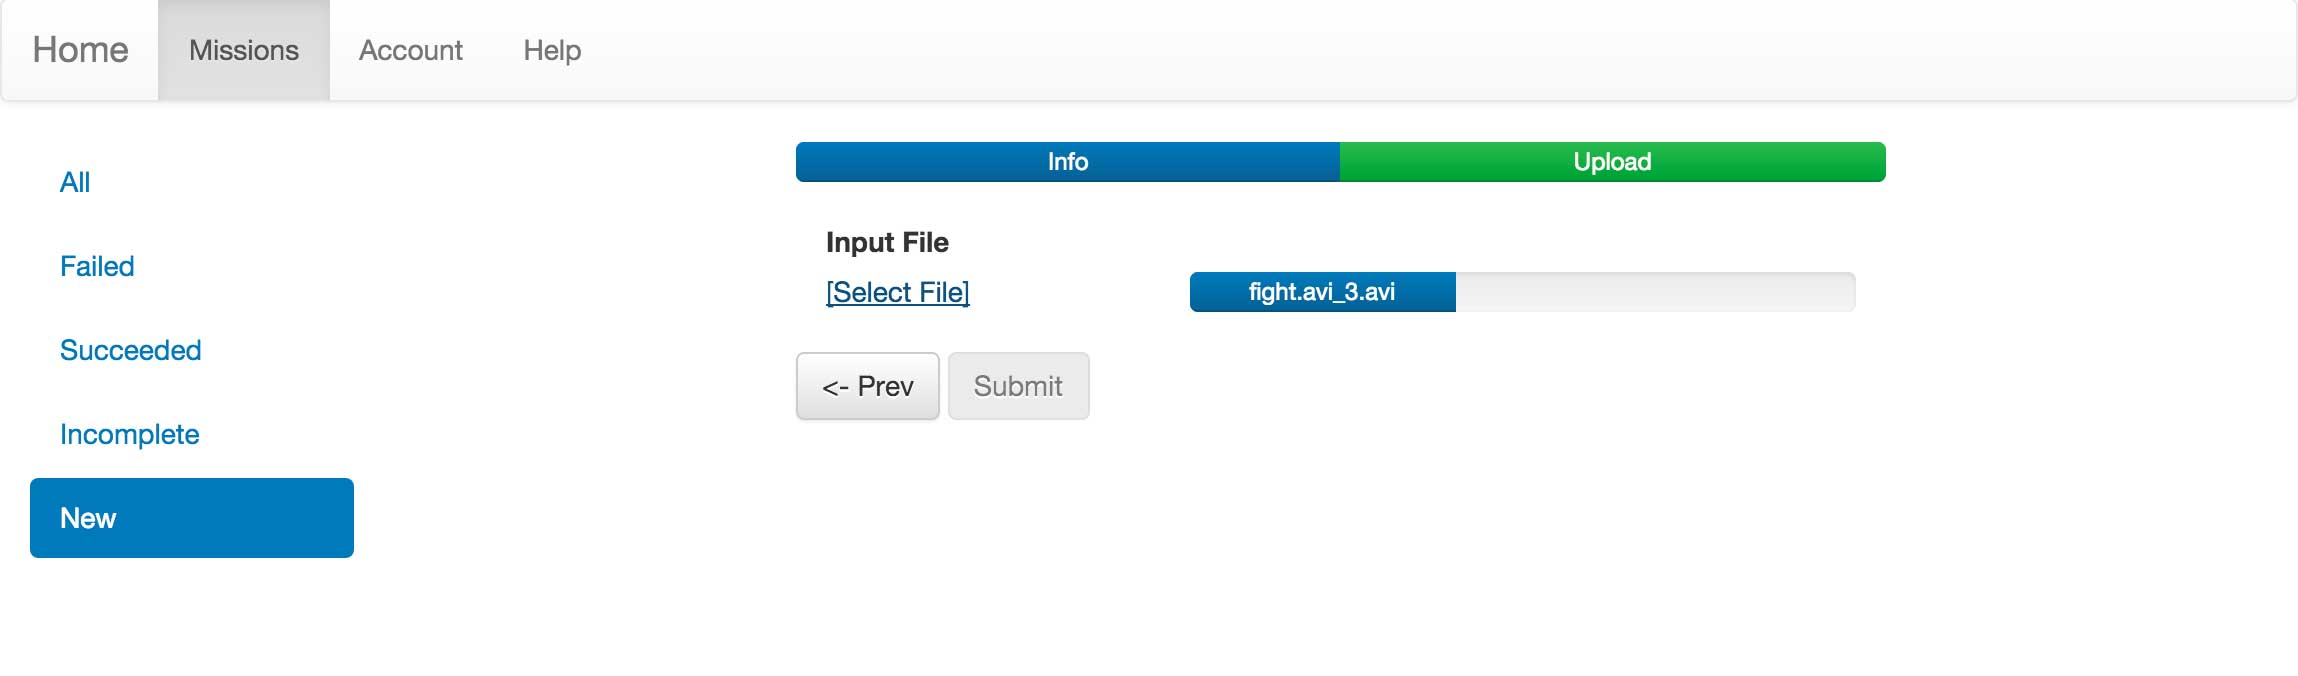
\includegraphics[width=0.8\textwidth]{website_upload_video}
\caption{上传果蝇行为视频}
\label{fig:website_upload_video}
\end{figure}

在此阶段,用户看到如图~\ref{fig:website_waiting_for_result}界面。

\begin{figure}
\centering
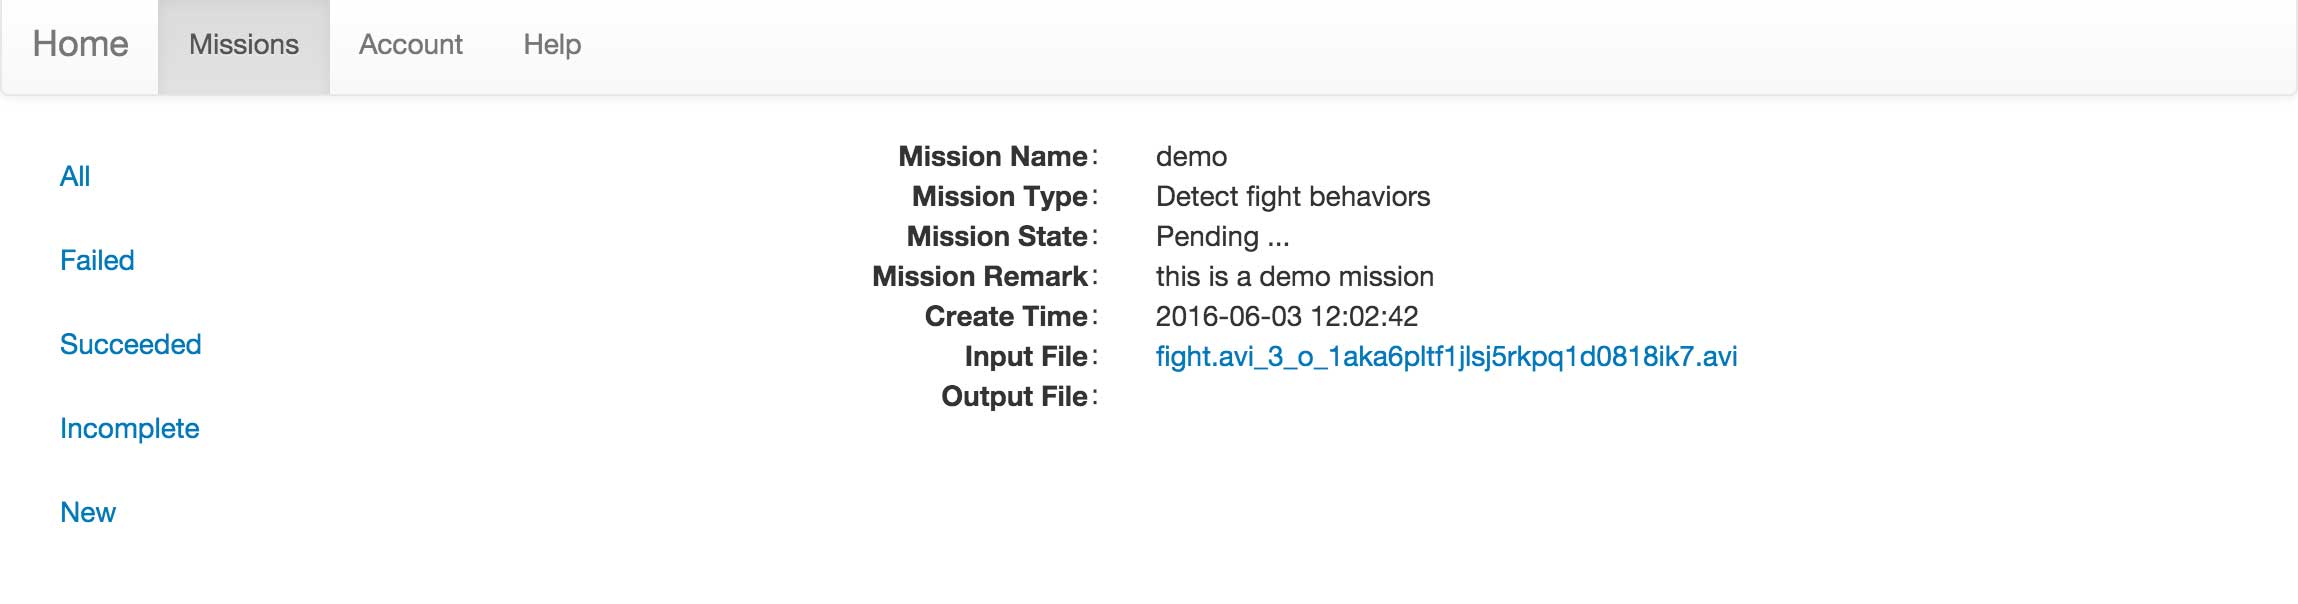
\includegraphics[width=0.8\textwidth]{website_waiting_for_result}
\caption{等待任务完成}
\label{fig:website_waiting_for_result}
\end{figure}

最后,经过任务队列的等待后,网站后台对任务进行分析,得到果蝇行为识别的结果,如图~\ref{fig:website_show_result}所示。

\begin{figure}
\centering
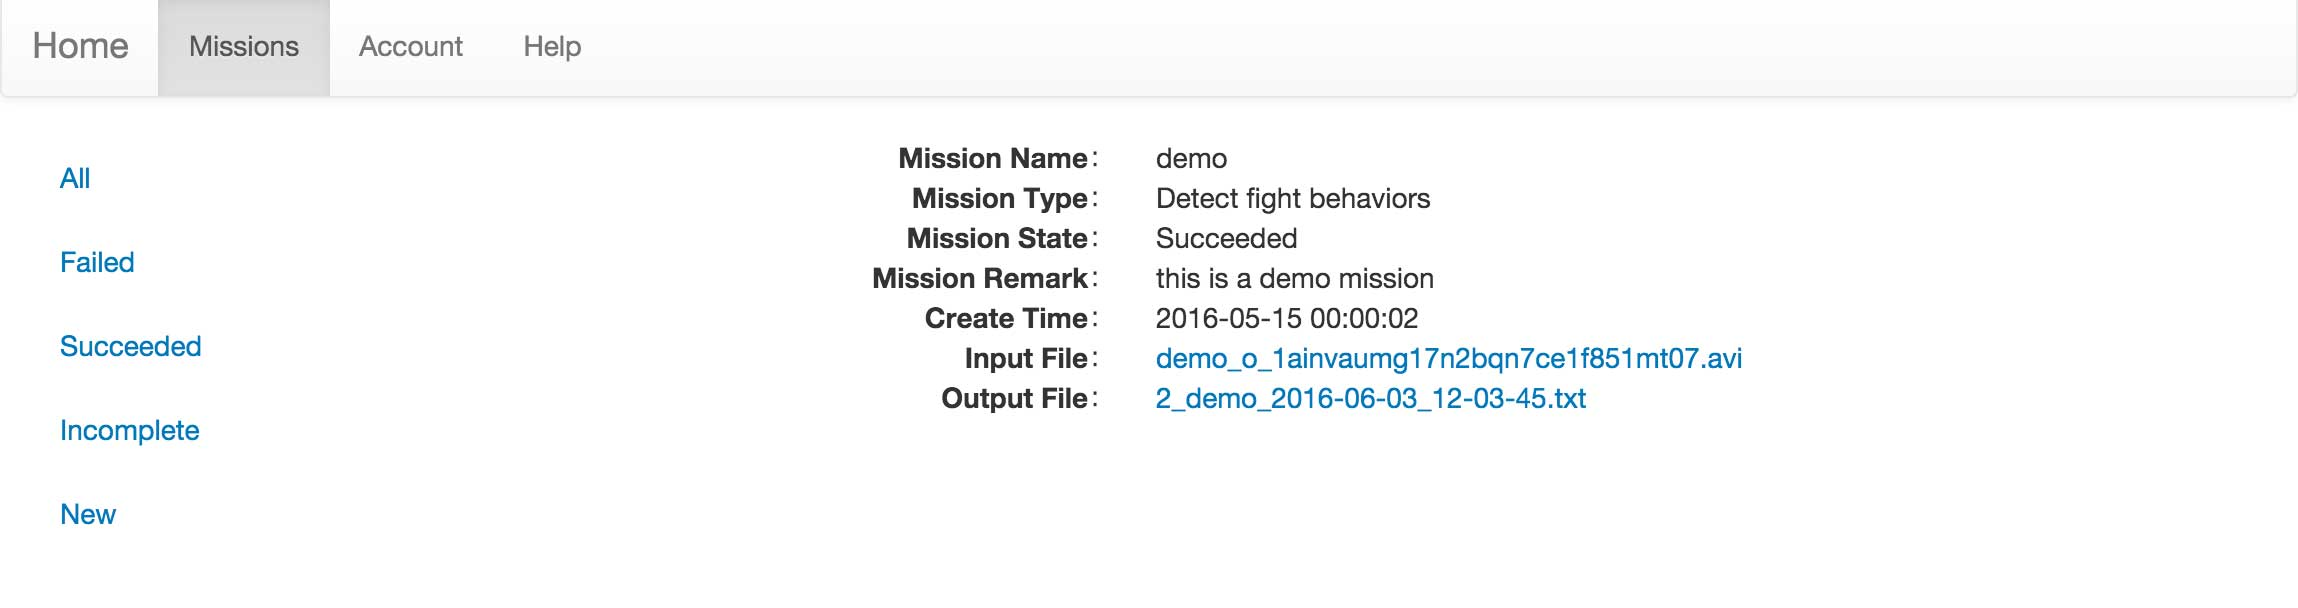
\includegraphics[width=0.8\textwidth]{website_show_result}
\caption{果蝇行为识别任务的结果}
\label{fig:website_show_result}
\end{figure}

图~\ref{fig:website_show_result}中,"Output File"栏目对应的就是果蝇行为识别的结果,即果蝇打架日志。对于不同类型的果蝇行为分析任务,其日志输出有不同的格式。对于打架行为,日志的第一行统计了视频中果蝇的打架次数,其后有以下3列:
\begin{itemize}
\item time – 打架发生的时间
\item frame – 打架发生的帧数,和time对应(从零开始)
\item strength – 打架强度
\end{itemize}
对于果蝇的求偶行为,求偶行为包括果蝇的身体求偶行为和振翅求偶行为,日志的第一行统计了视频中的求偶行为总数,其后有以下4列:
\begin{itemize}
\item time – 求偶起始时间
\item start – 求偶起始帧(含)
\item end – 求偶结束帧(含)
\item behavior – 求偶行为
\end{itemize}

除基本的日志外,果蝇求偶行为分析日志文件还输出简单的统计信息。在输出身体求偶或振翅求偶行为后,日志输出各求偶行为的持续时间,包括:
\begin{itemize}
\item count – 行为总发生次数
\item duration – 行为总持续时间
\end{itemize}
最后,日志输出行为间的转移矩阵,其第$i$行第$j$列表示从第$j$个行为向第$i$个行为转移的次数,单位为帧。用户通过下载果蝇行为日志文件,并按照既定格式进行分析,得到果蝇行为的各项参数,用于支持果蝇行为学的研究。

\subsection{果蝇行为识别网站简介}

网站建设在Ubuntu 14.04系统上,操作系统的选择主要考虑了果蝇行为识别程序的发布、网站服务的搭建等,最后综合选取了Ubuntu 14.04操作系统。网站的基本环境要求如下:
\begin{itemize}
    \item 操作系统:Ubunutu 14.04
    \item Web服务器: Apache2,支持PHP
    \item PHP: >=5.2.4
    \item 数据库:MySQL 5.5
    \item Python: 2.7.x
\end{itemize}

网站部分使用CodeIgniter框架搭建。CodeIgniter是一个轻量级的MVC架构的php网站框架,基于MVC模型,将网站的应用层和逻辑层进行分离\cite{burbeck87}。关于后台的数据库,系统使用MySQL数据库存储数据,主要存储了包括用户账户相关的数据表、任务类型数据表、任务数据表等,分别参见表~\ref{tab:account}、表~\ref{tab:mission_type}和表~\ref{tab:misson}。

\begin{table}
\centering
\caption{账户信息数据表dp\_account}
\label{tab:account}
\begin{tabular}{ccc}
\toprule[1.5pt]
字段名 & 字段类型 & 备注 \\ \midrule[1pt]
aid & bigint(20) & Unsigned, Primary key, Auto Increment \\
state & tinyint(4) & 0:等待审核,1:正常,2:禁用 \\
username & varchar(20) & 用户名 \\
password & varchar(32) & 密码的md5 \\
work\_unit & varchar(255) & 学校/单位 \\
department & varchar(255) & 院系 \\
purpose & varchar(255) & 实验目的 \\
source & varchar(255) & 项目来源 \\
data\_amount & varchar(255) & 数据量 \\
create\_time & timestamp & 默认current\_timestamp \\ \bottomrule[1.5pt]
\end{tabular}
\end{table}

\begin{table}
\centering
\caption{任务类型数据表dp\_missiontype}
\label{tab:mission_type}
\begin{tabular}{ccc}
\toprule[1.5pt]
字段名 & 字段类型 & 备注 \\ \midrule[1pt]
mtid & int(10) & Unsigned, Primary key, Auto Increment \\
state & tinyint(3) & 0:Invalid, 1:Valid \\
typename & varchar(255) & 类型名称 \\
description & varchar(1000) & 类型说明 \\
command & varchar(255) & 处理命令,可以加入特殊符号,具体见下表 \\
in\_file\_exts & varchar(255) & 允许的输入文件后缀,逗号分隔 \\
out\_file\_ext & varchar(10) & 输出文件的后缀 \\
max\_in\_file\_size & varchar(20) & 允许上传的输入文件大小 \\
error\_messages & varcahr(1000) & json格式字符串,各个error\_code的含义 \\ \bottomrule[1.5pt]
\end{tabular}
\end{table}

\begin{table}
\centering
\caption{任务数据表dp\_mission}
\label{tab:misson}
\begin{tabular}{ccp{0.5\columnwidth}}
\toprule[1.5pt]
字段名 & 字段类型 & 备注 \\ \midrule[1pt]
mid & bigint(20) & Unsigned, Primary key, Auto Increment \\
aid & bigint(20) & 所属account的aid \\
type & mediumint(6) & 任务类型的id,对应dp\_missiontype中的mtid \\
name & varchar(20) & 任务名称 \\
remark & varchar(1000) & 任务备注 \\
state & smallint(6) & {任务状态,
\begin{itemize}
    \item 0 : Pending等待处理
    \item 1 : Proceeding处理中
    \item 2 : Succeeded
    \item 3 : Failed
\end{itemize}} \\
error\_code & int(11) & 错误码,状态为Failed时有效 \\
in\_file\_path & varchar(255) & 输入文件路径,相对于项目根目录 \\
out\_file\_path & varchar(255) & 输出文件路径,相对于项目根目录,状态为Succeeded时有效 \\
stdout\_file\_path & varchar(255) & 处理过程的stdout日志文件路径,相对于项目根目录,状态为Succeeded/Failed时有效 \\
stderr\_file\_path & varchar(255) & 处理过程的stderr日志文件路径,相对于项目根目录,状态为Succeeded/Failed时有效 \\
create\_time & timestamp & 创建时间,默认current\_timestamp \\
complete\_time & datetime & 完成时间,状态为Succeeded/Failed时有效 \\
\bottomrule[1.5pt]
\end{tabular}
\end{table}

任务处理使用Python脚本实现,并用Supervisor管理脚本的执行。Supervisor是一个基于Python的进程管理系统,可以方便的进行任务的创建、监听、重启、崩溃恢复等,经过简单的配置后,可以用Supervisor进行任务队列的管理,安排果蝇自动检测程序DetectFly对果蝇视频的任务队列进行逐个分析和处理。通过为不同的任务类型指定不同的命令行参数,调用DetectFly程序,完成果蝇行为的识别,并将行为识别的结果保存为日志文件,方便用户下载和分析。

\section{小结}

在Ubuntu下配置开发环境,得到果蝇行为自动识别的可执行程序DetectFly。DetectFly可以通过命令行参数,实现不同类型的果蝇行为识别。在CodeIgniter框架的基础上,使用Supervisor进行任务队列管理,最终实现了果蝇行为识别网站的任务管理。
